\documentclass[journal,12pt,twocolumn]{IEEEtran}

\usepackage{setspace}
\usepackage{gensymb}

\singlespacing


\usepackage[cmex10]{amsmath}

\usepackage{amsthm}

\usepackage{mathrsfs}
\usepackage{txfonts}
\usepackage{stfloats}
\usepackage{bm}
\usepackage{cite}
\usepackage{cases}
\usepackage{subfig}

\usepackage{longtable}
\usepackage{multirow}

\usepackage{enumitem}
\usepackage{mathtools}
\usepackage{steinmetz}
\usepackage{tikz}
\usepackage{circuitikz}
\usepackage{verbatim}
\usepackage{tfrupee}
\usepackage[breaklinks=true]{hyperref}
\usepackage{graphicx}
\usepackage{tkz-euclide}
\usepackage{float}
\usepackage{blkarray}

\usetikzlibrary{calc,math}
\usepackage{listings}
    \usepackage{color}                                            %%
    \usepackage{array}                                            %%
    \usepackage{longtable}                                        %%
    \usepackage{calc}                                             %%
    \usepackage{multirow}                                         %%
    \usepackage{hhline}                                           %%
    \usepackage{ifthen}                                           %%
    \usepackage{lscape}     
\usepackage{multicol}
\usepackage{chngcntr}

\DeclareMathOperator*{\Res}{Res}

\renewcommand\thesection{\arabic{section}}
\renewcommand\thesubsection{\thesection.\arabic{subsection}}
\renewcommand\thesubsubsection{\thesubsection.\arabic{subsubsection}}

\renewcommand\thesectiondis{\arabic{section}}
\renewcommand\thesubsectiondis{\thesectiondis.\arabic{subsection}}
\renewcommand\thesubsubsectiondis{\thesubsectiondis.\arabic{subsubsection}}


\hyphenation{op-tical net-works semi-conduc-tor}
\def\inputGnumericTable{}                                 %%

\lstset{
%language=C,
frame=single, 
breaklines=true,
columns=fullflexible
}
\begin{document}


\newtheorem{theorem}{Theorem}[section]
\newtheorem{problem}{Problem}
\newtheorem{proposition}{Proposition}[section]
\newtheorem{lemma}{Lemma}[section]
\newtheorem{corollary}[theorem]{Corollary}
\newtheorem{example}{Example}[section]
\newtheorem{definition}[problem]{Definition}

\newcommand{\BEQA}{\begin{eqnarray}}
\newcommand{\EEQA}{\end{eqnarray}}
\newcommand{\define}{\stackrel{\triangle}{=}}
\bibliographystyle{IEEEtran}
\providecommand{\mbf}{\mathbf}
\providecommand{\pr}[1]{\ensuremath{\Pr\left(#1\right)}}
\providecommand{\qfunc}[1]{\ensuremath{Q\left(#1\right)}}
\providecommand{\sbrak}[1]{\ensuremath{{}\left[#1\right]}}
\providecommand{\lsbrak}[1]{\ensuremath{{}\left[#1\right.}}
\providecommand{\rsbrak}[1]{\ensuremath{{}\left.#1\right]}}
\providecommand{\brak}[1]{\ensuremath{\left(#1\right)}}
\providecommand{\lbrak}[1]{\ensuremath{\left(#1\right.}}
\providecommand{\rbrak}[1]{\ensuremath{\left.#1\right)}}
\providecommand{\cbrak}[1]{\ensuremath{\left\{#1\right\}}}
\providecommand{\lcbrak}[1]{\ensuremath{\left\{#1\right.}}
\providecommand{\rcbrak}[1]{\ensuremath{\left.#1\right\}}}
\theoremstyle{remark}
\newtheorem{rem}{Remark}
\newcommand{\sgn}{\mathop{\mathrm{sgn}}}
\providecommand{\abs}[1]{\vert#1\vert}
\providecommand{\res}[1]{\Res\displaylimits_{#1}} 
\providecommand{\norm}[1]{\lVert#1\rVert}
%\providecommand{\norm}[1]{\lVert#1\rVert}
\providecommand{\mtx}[1]{\mathbf{#1}}
\providecommand{\mean}[1]{E[ #1 ]}
\providecommand{\fourier}{\overset{\mathcal{F}}{ \rightleftharpoons}}
%\providecommand{\hilbert}{\overset{\mathcal{H}}{ \rightleftharpoons}}
\providecommand{\system}{\overset{\mathcal{H}}{ \longleftrightarrow}}
	%\newcommand{\solution}[2]{\textbf{Solution:}{#1}}
\newcommand{\solution}{\noindent \textbf{Solution: }}
\newcommand{\cosec}{\,\text{cosec}\,}
\providecommand{\dec}[2]{\ensuremath{\overset{#1}{\underset{#2}{\gtrless}}}}
\newcommand{\myvec}[1]{\ensuremath{\begin{pmatrix}#1\end{pmatrix}}}
\newcommand{\mydet}[1]{\ensuremath{\begin{vmatrix}#1\end{vmatrix}}}
\numberwithin{equation}{subsection}
\makeatletter
\@addtoreset{figure}{problem}
\makeatother
\let\StandardTheFigure\thefigure
\let\vec\mathbf
\renewcommand{\thefigure}{\theproblem}
\def\putbox#1#2#3{\makebox[0in][l]{\makebox[#1][l]{}\raisebox{\baselineskip}[0in][0in]{\raisebox{#2}[0in][0in]{#3}}}}
     \def\rightbox#1{\makebox[0in][r]{#1}}
     \def\centbox#1{\makebox[0in]{#1}}
     \def\topbox#1{\raisebox{-\baselineskip}[0in][0in]{#1}}
     \def\midbox#1{\raisebox{-0.5\baselineskip}[0in][0in]{#1}}
\vspace{3cm}
\title{Assignment 8}
\author{Satya Sangram Mishra}
\maketitle
\newpage
\bigskip
\renewcommand{\thefigure}{\theenumi}
\renewcommand{\thetable}{\theenumi}
Download all python codes from 
\begin{lstlisting}
https://github.com/satyasm45/Summer-Internship/tree/main/Assignment-8/Codes
\end{lstlisting}
%
and latex-tikz codes from 
%
\begin{lstlisting}
https://github.com/satyasm45/Summer-Internship/tree/main/Assignment-8
\end{lstlisting}
%
\section{Question No. 2.64}
In a legislative assembly election, a political
group hired a public relations firm to promote
its candidate in three ways: telephone, house
calls, and letters. The cost per contact (in paise)
is given in matrix $\vec{A}$ as
\begin{center}
Cost per Contact(in Paise)
\end{center}
\begin{align}
    \vec{A}=
    \begin{blockarray}{cc}
    \text{cost}\\
    \begin{block}{(c)(c)}
    40 &\text{Telephone}\\
    100&\text{Housecall} \\
    50&\text{Letter}\\
    \end{block}
    \end{blockarray}
\end{align}
The number of contacts of each type made in
two cities X and Y is given by matrix $\vec{B}$
\begin{align}
    \vec{B} =
    \begin{blockarray}{cccc}
    \text{Telephone} & \text{Housecall} & \text{Letter} \\
    \begin{block}{(ccc)(c)}
    1000 & 500 & 5000 & \text{X}\\
    3000 & 1000 & 10000 & \text{Y} \\
    \end{block}
    \end{blockarray}
\end{align}
Find the total
amount spent by the group in the two cities
X and Y
\section{Explanation}
The total amount spent is given by=

    \begin{align}
    \vec{B}\vec{A}\\
    =\myvec{1000&500&5000\\3000&1000&10000}\myvec{40\\100\\50}\\
    =\myvec{40000+50000+250000\\120000+100000+500000}\\
    \begin{blockarray}{cc}
    \text{TotalCost} \\
    \begin{block}{(c)(c)}
    340000&\text{X}\\
    720000&\text{Y}\\
    \end{block}
    \end{blockarray}
    \end{align}
$\therefore$ the total amount spent in city X and city Y is 3400 and 7200 Rupees respectively.

\numberwithin{figure}{section}
\begin{figure}[!ht]
\centering
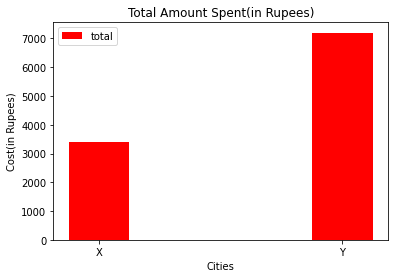
\includegraphics[width=\columnwidth]{figure8}
\caption{Total Amount Spent by the group in cities X and Y}
\label{fig:Profit}	
\end{figure}
\end{document}